\documentclass[dvipdfmx]{jsarticle}
\usepackage[dvipdfmx]{graphicx}
\usepackage{amsmath, amssymb}
\usepackage{mathtools}
\usepackage{here}

\begin{document}
\title{卒業論文回答}
\author{権藤陸}
\maketitle
\section{山中先生のご質問に対する回答}
\subsection{レーダのキャリブレーションとは何か}
一定時間毎に行われる,より正確なアークタンジェント復調を行うためのDCオフセット補償です.
レーダによる測定中に,受信機の不完全性やクラッタ反射によるDCオフセットの誤差が発生するため,その誤差を補償することでI/Q信号を補正します.受信機の不完全性には,サーキュレータの絶縁、アンテナのミスマッチ、ミキサーのLOとRFポートの絶縁などがあります\cite{calibration}.
一定時間ごとにキャリブレーションを行う理由として,今回の実験環境では,測定中に被験者が動き,クラッタが変化することによるDCオフセット誤差の変化が挙げられます.

\subsection{ノイズの多いデータセットに含まれるノイズとは何か}
ここでは,心拍周波数の真値である0.75-1.05 Hzの信号を取得したい信号,それ以外の周波数帯の信号をノイズとする.0.75Hz未満のノイズは,主に被験者の体動や呼吸,前述のキャリブレーション,ベッドや周辺にある物体からのクラッタなどに起因するものと考えられます.
他にノイズの内訳として,ベッドの振動,受信機の熱雑音によるノイズ,レーダ自体が振動により動いてしまうことで発生するドップラー,同一周波数帯の電波源からの干渉などが考えられますが,これらのノイズの周波数帯を特定することは困難であると考えられます.

\subsection{ウェーブレット再構成で除かれたノイズについて}
以下にウェーブレット再構成前後におけるWelch法で得た周波数特性(0-2.0Hz)の図を示します.縦線は心拍周波数の真値の最小値と最大値を示します.
次の式で定義するウェーブレット再構成前と後の平均パワー比を求めると,
\begin{equation}\label{}
平均パワー比 = \frac{0-0.75 \mathrm{Hz}の平均パワー}{0.75-1.05 \mathrm{Hz}の平均パワー}
\end{equation}

前述のように,心拍周波数の真値0.75-1.05 Hz以外の周波数帯の信号をノイズとする.特にウェーブレット再構成では,0.75 Hz未満の周波数帯,すなわち体動や呼吸に起因すると考えられるノイズに注目します.
ウェーブレット再構成前は平均パワー比が452.4, ウェーブレット再構成後は平均パワー比が4.0で,再構成後の方がパワー比が約1/113になり,0.75Hz未満のノイズの影響が再構成により小さくなったため,モデルの学習が安定し,良い精度につながったのではないかと考えられます.

\begin{figure}[htbp]
    \begin{minipage}[c]{0.5\hsize}
      \centering
      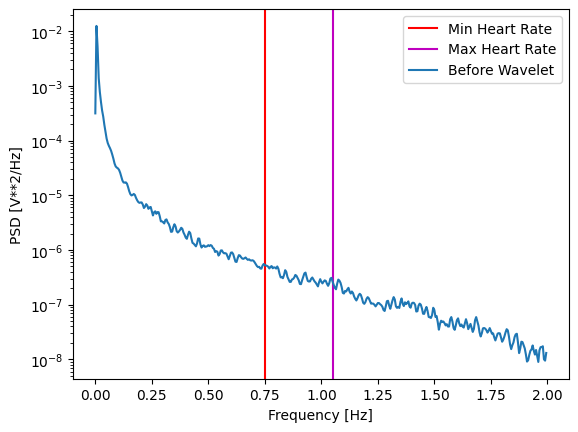
\includegraphics[width=\linewidth]{./fig/before_wavelet_freq.png}
      \caption{ウェーブレット再構成前の周波数特性(Welch法)}
    %   \label{fig:statue}
    \end{minipage}
    \begin{minipage}[c]{0.5\hsize}
      \centering
      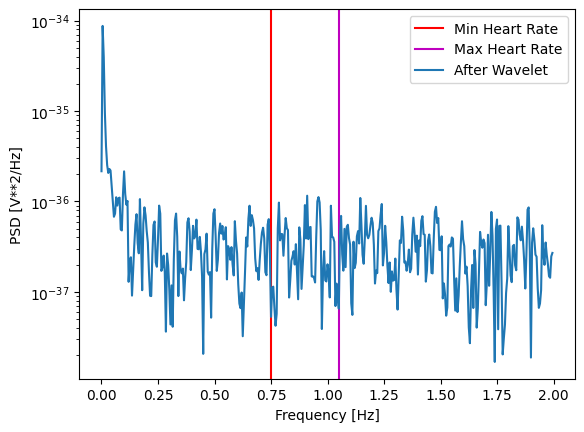
\includegraphics[width=\linewidth]{./fig/after_wavelet_freq.png}
      \caption{ウェーブレット再構成後の周波数特性(Welch法)}
    %   \label{fig:spaceship}
    \end{minipage}
\end{figure}

\begin{table}[H]
\caption{Welch法のパラメータ}
\centering
\begin{tabular}{cc}
\hline
全体のウィンドウサイズ & 200000 \\
セグメントあたりのポイント数 & 50000 \\
オーバーラップ & 25000 \\
周波数分解能(Hz) & 0.005 \\
サンプリングレート(s) & 250 \\
\hline
\end{tabular}
\end{table}

\section{寺岡先生のご質問に対する回答}
\subsection*{被験者が増えた時にモデルの識別時間はどれほど増えるか}
12人と30人の識別しか試せておらず、より多くの人数によるセグメントあたりの識別時間の変化を実験的に確かめることはできませんが,計算量の観点から言えば、10万人のデータセットでもモデルサイズと入力セグメントのサイズが同じであれば、計算量が同じため、識別時間も同じと考えられます。

また,ご質問の中で寺岡先生がこれはシミュレーションかと尋ねられた際に,私はシミュレーションですとお答えしましたが,入力に用いたデータは実験で得たものですので,シミュレーションではございません.こちらで訂正させていただきます.

\begin{thebibliography}{99}
    \bibitem{calibration} B. -K. Park, O. Boric-Lubecke and V. M. Lubecke, "Arctangent Demodulation With DC Offset Compensation in Quadrature Doppler Radar Receiver Systems," in IEEE Transactions on Microwave Theory and Techniques, vol. 55, no. 5, pp. 1073-1079, 2007
\end{thebibliography}

\end{document}